\documentclass[a4paper,12pt,openany,oneside]{article}
\def\pdfglyphtounicode#1#2{}
%______________________________________IMPORTATION DES PACKAGES_________________________________________




%mise en page
\usepackage{layout}     
\usepackage[top=2cm, bottom=2cm, left=2cm, right=2cm]{geometry}
\usepackage{setspace}
\usepackage{lscape}
\usepackage{fancyhdr}
\renewcommand{\baselinestretch}{1.2}
%\usepackage{ulem}
\usepackage{enumitem}
\usepackage{lipsum}
\usepackage{datetime}				
% custom date
\newdateformat{mydate}{\monthname[\THEMONTH] \THEYEAR}	

%Gloossaire
%\usepackage[automake]{glossaries}
%\makeglossaries
%\setglossarystyle{listgroup}

%Couleurs
\usepackage{color}
\definecolor{BleuFonce}{RGB}{0,74,117}
\usepackage[usenames,dvipsnames]{xcolor}
\usepackage{colortbl}

%______________________________________POLICES ET ACCENTS_________________________________________
\usepackage{ifxetex}
\ifxetex
    \usepackage{fontspec}
    \setmainfont{Latin Modern Roman}
    \setsansfont{Latin Modern Sans}
    \setmonofont{Latin Modern Mono}
\else
    \usepackage[T1]{fontenc}
    \usepackage[utf8]{inputenc}
    \usepackage{lmodern}
\fi
\usepackage[french]{babel}
\usepackage{amsfonts}

% Force proper font encoding for PDF - CRUCIAL for correct accent rendering
% \input{glyphtounicode}
% \pdfgentounicode=1


%maths et symboles
\usepackage{amsmath}
\usepackage{amssymb}
\usepackage{pifont}
\usepackage{dsfont}
\usepackage{chemarr}

%insertion images et graphiques
\usepackage{graphicx,subfigure}
%\usepackage{graphicx}
\usepackage{wrapfig}
\usepackage{wasysym}
\usepackage{tikz}
\usepackage{chemfig}
 \usepackage{tikz,pgfplots}
\usepackage[framemethod=tikz]{mdframed}
\usetikzlibrary{shadows,shadings}

%tableaux
\usepackage{multirow}
\usepackage{multicol}
\usepackage{makecell}
\setcellgapes{6pt}

%Liens et PDF
% \usepackage{minitoc}
\usepackage[bookmarks=true,bookmarksnumbered=true]{hyperref}
\usepackage{url}


%Informatique et code source
\usepackage{listings}

%%configuration de listings
\lstset{
language=python,
basicstyle=\ttfamily\small, %
identifierstyle=\color{red}, %
keywordstyle=\color{blue}, %
stringstyle=\color{black!60}, %
commentstyle=\it\color{green!95!yellow!1}, %
columns=flexible, %
tabsize=2, %
extendedchars=true, %
showspaces=false, %
showstringspaces=false, %
numbers=left, %
numberstyle=\tiny, %
breaklines=true, %
breakautoindent=true, %
captionpos=b
}


%%%%%%%%%%%%%%%%%%%%%%%%%%%% Tahiry   %%%%%%%%%%%%%%%%%%%%%%%
\usepackage[most]{tcolorbox} % For problem answer sections
%\graphicspath{ {./Theme_LaTeX/Icones/} }
\graphicspath{ {./Icones/} }
% \usepackage{pythonhighlight}

%%%%%%%%%%%%%%%%%%%%%%%%%%%%%%%%fond de page %%%%%%%%%%%%%%%%%%%%%%%
\usepackage{eso-pic,graphicx}
\usepackage{xcolor}
\newcommand{\bgimg}[1]{
\AddToShipoutPicture
	{
		\put(\LenToUnit{0 cm},\LenToUnit{0.0\paperheight})
		{
				\includegraphics[width=\paperwidth,height=\paperheight]{#1} 
		}
	}
}


%______________________

%_______________________________________________________________________________
%_______________________________________________________________________________





%_____________________________________PAGE DE GARDE : COURS(Book)_____________
\newcommand\PageDeGardeCours[3]{
\addto\captionsfrench{\renewcommand{\chaptername}{Chapitre n°  \hspace{0.1cm}\Large{n°} }}

	\makeatletter
	\begin{titlepage}
		
		\begin{flushright}
			\today
		\end{flushright}
		\vspace{3cm}
		\begin{center}
			\Huge{#1}
			
			\vspace{2cm}
			\begin{figure}[h]
				\centering
				
\includegraphics[width=10cm]{image_Cours}
			\end{figure}
			\vspace{1cm}
			\normalsize{\itshape Support de cours : #3}
			
			
			\vspace{\fill}\itshape
			\textcolor{Gray}{ #2}
			\vspace{\fill}
		\end{center}
	\end{titlepage}
	
	\newpage
	
%--TABLES DES MATERES & Co. 
\makeatother
\setcounter{tocdepth}{0}
\dominitoc%
\tableofcontents
\listoffigures
\newpage
\listoftables
\newpage

}

%_____________________________________PAGE DE GARDE : TP (Book)_____________
\newcommand\PageDeGardeTP [3]{
\addto\captionsfrench{\renewcommand{\chaptername}{T.P  \hspace{0.1cm}\Large{n°} }}

	\makeatletter
	\begin{titlepage}
		
		\begin{flushright}
			\today
		\end{flushright}
		\vspace{3cm}
		\begin{center}
			\Huge{#1}
			
			\vspace{2cm}
			\begin{figure}[h]
				\centering
				
\includegraphics[width=10cm]{image_TP}
			\end{figure}
			\vspace{1cm}
			\normalsize{\itshape Support de Travaux Pratiques : #3}
			
			
			\vspace{\fill}\itshape
			\textcolor{Gray}{ #2}
			\vspace{\fill}
		\end{center}
	\end{titlepage}
	
	\newpage
	
%--TABLES DES MATERES & Co. 
\makeatother
\setcounter{tocdepth}{0}
\dominitoc
\tableofcontents
\listoffigures
\newpage
\listoftables
\newpage

}
%_____________________________________PAGE DE GARDE : TD (Book)_____________
\newcommand\PageDeGardeTD [3]{
\addto\captionsfrench{\renewcommand{\chaptername}{T.D  \hspace{0.1cm}\Large{n°} }}

	\makeatletter
	\begin{titlepage}
		
		\begin{flushright}
			\today
		\end{flushright}
		\vspace{3cm}
		\begin{center}
			\Huge{#1}
			
			\vspace{2cm}
			\begin{figure}[h]
				\centering
				
\includegraphics[width=10cm]{image_TD}
			\end{figure}
			\vspace{1cm}
			\normalsize{\itshape Recueil d'exercices : #3}
			
			
			\vspace{\fill}\itshape
			\textcolor{Gray}{ #2}
			\vspace{\fill}
		\end{center}
	\end{titlepage}
	
	\newpage
	
%--TABLES DES MATERES & Co. 
\makeatother
\setcounter{tocdepth}{0}
\dominitoc
\tableofcontents
\listoffigures
\newpage
\listoftables
\newpage

}
%_____________________________________PAGE DE GARDE : Annales (Book)_____________
\newcommand\PageDeGardeAnnales [3]{
\addto\captionsfrench{\renewcommand{\chaptername}{T.D  \hspace{0.1cm}\Large{n°} }}

	\makeatletter
	\begin{titlepage}
		
		\begin{flushright}
			\today
		\end{flushright}
		\vspace{3cm}
		\begin{center}
			\Huge{#1}
			
			\vspace{2cm}
			\begin{figure}[h]
				\centering
				
\includegraphics[width=10cm]{image_Exam}
			\end{figure}
			\vspace{1cm}
			\normalsize{\itshape Recueil d'examens : #3}
			
			
			\vspace{\fill}\itshape
			\textcolor{Gray}{ #2}
			\vspace{\fill}
		\end{center}
	\end{titlepage}
	
	\newpage
	
%--TABLES DES MATERES & Co. 
\makeatother
\setcounter{tocdepth}{0}
\dominitoc
\tableofcontents
\listoffigures
\newpage
\listoftables
\newpage

}

%_____________________________________PAGE DE GARDE : Partiel (Article)_____________
\newcommand\PageDeGardePartiel [3]{
\makeatletter 
\def\thickhrulefill{\leavevmode \leaders \hrule height 1pt\hfill \kern \z@} 
\renewcommand{\maketitle}{\begin{titlepage}% 
		\let\footnotesize\small 
		\let\footnoterule\relax 
		\parindent \z@ 
		\reset@font 
		\null 
		\vskip 0\p@ 
		\hbox{\mbox{\hspace{3em}}% 
			\vrule depth 0.6\textheight% 
			\mbox{\hspace{2em}} 
			\vbox{ 
				\vskip 30\p@ 
				\begin{flushleft} 
					\Large \@author \par 
				\end{flushleft} 
				\vskip 40\p@ 
				\begin{flushleft} 
					\huge \bfseries \@title \par 
				\end{flushleft} 
				\vskip 5\p@ 
				\begin{flushleft} 
					\@date 
				\end{flushleft} 
				\vfil 
		}} 
		\null 
	\end{titlepage}% 
	\setcounter{footnote}{0}% 
} 
\makeatother 
\author{Devoir   \newline Durée : #2 \newline \textbf{Calculatrice programmable autorisée}} 
\title{#1} 
\date{ #3} 
	
%--TABLES DES MATERES & Co. 
\makeatother
\setcounter{tocdepth}{0}
\dominitoc
\tableofcontents
\listoffigures
\newpage
\listoftables
\newpage

}


%_____________________________PAGE DE GARDE : Rapport (Template Polytech )_____________
\newcommand\PageDeGardeRapport[5]{
\begin{titlepage}


%\thispagestyle{empty}

\newgeometry{left=6cm,bottom=2cm, top=1cm, right=1cm}

\tikz[remember picture,overlay] \node[opacity=1,inner sep=0pt] at (2.2mm,-165mm){
\includegraphics{fond1.png}}; % fond changeable 

% fonte sans empattement pour la page de titre

\color{white}

%%Texte vertical à gauche
\begin{picture}(0,0)
%\put(-110,-743){\rotatebox{90}{\Huge{#1}}}
\end{picture}
 
%**************************************************************
%********************  LOGO  DE  POLYTECH  ********************
%****** CHANGER L'IMAGE POUR UN AUTRE POLYTECH QUE SACLAY *****
%* VOIR LES LOGOS DISPONIBLES, ET REMPLACER LE NOM CI-DESSOUS *
%**************************************************************

\vspace{-10mm} % à ajuster en fonction de la hauteur du logo
               % décalera le texte en dessous
\flushright 
\includegraphics[width=50mm]{LOGO.png} % nom du logo du polytech




%*****************************************************
%******************** TITRE **************************
%*****************************************************
\flushright
\vspace{10mm} % à régler éventuellement
\color{BleuFonce}
\fontfamily{lmss}\fontseries{m}\fontsize{22}{26}\selectfont
 #1

\normalsize
\color{black}
%*****************************************************

%\fontfamily{fvs}\fontseries{m}\fontsize{8}{12}\selectfont

\vspace{1.5cm}
\normalsize

\textbf{Professeur référent : #2}

\vspace{15mm}

ECOLE : ESIROI \\  %% nom école
\small Spécialité : #3 \\  %% nom spécialité / enseignement

\vspace{15mm}

\textbf{#4}\\
\bigskip
\Large {\color{BleuFonce} \textbf{#5}}
\vspace{90mm}
\flushright 
\includegraphics[width=40mm]{LOGO_UR.png} % nom du logo UR
\end{titlepage}

\newpage
\newgeometry{left=2cm,bottom=2cm, top=2cm, right=2cm}
}
%%%%%%%%%%%%%%%%%%%%%%%%%%%%%%%%%%%%%%%%%%%%%%%%%%%%%%%%%%%%%%


%________________________________Page de cloture ___________________-
\newcommand\ClotureRapport [0]{
\newpage
\thispagestyle{empty}
.

\fontfamily{lmss}\fontseries{m}\selectfont

\small




%************************************
\vspace{\fill} % ALIGNER EN BAS DE PAGE
%************************************

% Modifier en fonction de l'école
\noindent
\color{BleuFonce} \footnotesize 
ESIROI \\
40 Avenue de Soweto\\
97410 Saint-Pierre, La Réunion
}

%------------------------------------EN TETE et bas de pages commun-----------
\pagestyle{fancy}
\lfoot{\textcolor{Gray}{\textit{\auteur}}}
\lhead{
\includegraphics[width=2cm]{LOGO_UR.png}}
\rhead{
\includegraphics[width=2cm]{LOGO.png}}
\rfoot{\thepage}



%___________________________________BAS DE PAGE PROPRE AU DOC____________
\chead{\textcolor{Gray}{\titre}}
% \cfoot{\textcolor{Gray}{\niveau}}
\cfoot{}
%---------------------------------------------------------------

%Encadré A retenir
\newcounter{theorem}%A modifier un jour où j'aurais du temps...

\renewcommand\thetheorem{}
\makeatletter
\mdf@dolist{\mdf@do@stringoption}{%
    {theoremtitle=={}}%
}
\renewrobustcmd\mdfcreateextratikz{%
      \node[anchor=west,rounded corners,draw,thick,shading=axis,left color=red!20,xshift=1cm,minimum height=.7cm,minimum width=2cm] at (P-|O) 
              {~\mdf@frametitlefont{\thetheorem}%
                  \ifdefempty{\mdf@theoremtitle}%
                  {~}%
                  {~\mdf@theoremtitle~}%
              };
}
\makeatother
\mdfdefinestyle{theoremstyle}{
outerlinewidth=1pt,
innerlinewidth=0pt,
roundcorner=2pt,
linecolor=black,
shadow=true,
tikzsetting={shading=axis,top color=orange!20},
innertopmargin=1.2\baselineskip,
skipabove={\dimexpr0.5\baselineskip+\topskip\relax},
needspace=3\baselineskip,
frametitlefont=\sffamily\bfseries,
settings={\global\stepcounter{theorem}},
}
\newenvironment{retenir}[1][]
{\begin{mdframed}[style=theoremstyle,theoremtitle={#1}]\relax}{\end{mdframed}}




%______________________________FORMATAGE DES TITRES_____________________
\newcommand\Chapitre [1]{\textcolor{Mahogany} {\chapter{\bfseries #1}}}
\newcommand\TitreA [1]{\textcolor{Mahogany} {\section{\bfseries #1}}}
\newcommand\TitreB [1]{{\addtolength{\leftskip}{1cm}\textcolor{MidnightBlue} {\subsection{\itshape #1}}}}
\newcommand\TitreC [1]{{\addtolength{\leftskip}{1,5cm}\textcolor{Sepia} {\subsubsection{ \RIGHTarrow    #1}}}}
\newcommand\TitreAb [1]{\textcolor{Mahogany} {\section*{\bfseries #1}}}
\newcommand\TitreBb [1]{{\addtolength{\leftskip}{1cm}\textcolor{MidnightBlue} {\subsection*{\itshape #1}}}}
\newcommand\TitreCb [1]{{\addtolength{\leftskip}{1,5cm}\textcolor{SeaGreen} {\subsubsection*{\itshape #1}}}}
\newcommand{\Exo}[1]
{{\textcolor{Sepia}{\large \textbf{\stepcounter{cexercice} Exercice n°\arabic{cexercice} : #1}\\}}}
\newcommand\Retenir[1]{ \vspace{1cm}\textcolor{RedOrange} {{ \fontfamily{augie}\selectfont #1\vspace{1cm} }}}
%---------------------------------------------------------------



%____________________________FORMAT Encadrés et surlignés___________________________

 \definecolor{light-gray}{gray}{0.95}

\newcommand{\Encadre}[1]
{
\fcolorbox{gray}{light-gray}{
\begin{minipage}{0.9\textwidth}
#1
\end{minipage}
}
}

\definecolor{light-gray}{rgb}{0.98,0.98,0.98}
\newcommand{\CadreG}[1]{
\fcolorbox{black}{light-gray}{\begin{minipage}[c]{0.95\linewidth}
\vspace{0.2cm}
#1

\end{minipage}}
\vspace{0.2cm}
}

\definecolor{powderblue}{rgb}{0.69, 0.88, 0.9}
\newcommand{\CadreB}[1]{
\fcolorbox{black}{powderblue}{\begin{minipage}[c]{0.95\linewidth}
\vspace{0.2cm}
#1

\end{minipage}}
\vspace{0.2cm}
}
  
\newcommand{\EtiquetteR}[1]
   {\vspace{0.5cm}\colorbox{GreenYellow}{\textcolor{RedOrange}{\textbf{#1}}}\vspace{0.5cm}}

\newcommand{\BoiteColor}[3]
   {\colorbox{#1}{\textcolor{#2}{\large{\textbf{#3}}}}}
   
% \newcommand\Smile[0]{\begin{center} \blacksmiley\end{center}}
%_______________________________________________________________________________

%_________________________________________Formattage article court_____________________
% Define separators
\newcommand{\HorRule}[1]{\noindent\rule{\linewidth}{#1}} % Creating a horizontal rule
\newcommand{\SepRule}{\noindent							 % Creating a separator
						\begin{center}
							\rule{250pt}{1pt}
						\end{center}
						}						

% Define Title en News input
\newcommand{\JournalName}[1]{%
		\begin{center}	
			\Huge \usefont{T1}{augie}{m}{n}
			#1%
		\end{center}	
		\par \normalsize \normalfont}
		
\newcommand{\JournalIssue}[1]{%
		\hfill \textsc{\mydate \today}
		\par \normalsize \normalfont}

\newcommand{\NewsItem}[1]{%
		\usefont{T1}{augie}{m}{n} 	
		\large #1 \vspace{4pt}
		\par \normalsize \normalfont}
		
\newcommand{\NewsAuthor}[1]{%
			\hfill by \textsc{#1} \vspace{4pt}
			\par \normalfont}		



%____________________________FORMAT QCM___________________________
\newcommand{\Trou}[0]
   {........................ }

\newcommand{\Question}[0]
   {\begin{wrapfigure}[2]{l}{10mm}\vspace{-0.6cm}\includegraphics{Figs/Question.png}\end{wrapfigure}}

\newcommand{\Reponse}[1]
   {{\textcolor{PineGreen}{\textit{#1}}}}
%_______________________________________________________________________________


%____________________________FORMAT VECTEURS en MECA___________________________

\newcommand{\vecteur}[3]
{
\[
\vec{#1}
\left \{
   \begin{array}{r c l}
      #1_x & = & #2\\
     #1_y & = & #3 \\
   \end{array}  \right .
\]
}
\newcommand{\OM}[2]
{
\[
\vec{OM}
\left \{
   \begin{array}{r c l}
      x(t) & = & #1\\
     y(t) & = & #2 \\
   \end{array}  \right .
\]
}
%_______________________________________________________________________________



%____________________________FORMAT MOLECULES & Co. en CHIMIE__________________________

\newcommand{\Molecule}[1]
{
\chemfig{[,0.7]#1}
}
\newcommand{\FlecheRea}[2]
{
\xrightarrow[   #1   ]{#2}\hspace{0.5cm}
}
\newcommand{\Meso}[0]
{
\hspace{5mm}
\longleftrightarrow
\hspace{5mm}
}
\newcommand{\electron}[0]{
$e^-$
}

	
%________________________________________________Compétences__________________________________
\newcommand{\RCO}[0]
   {\colorbox{Yellow}{\textcolor{black}{\textbf{RCO}}}\vspace{0.2cm}}
\newcommand{\APP}[0]
   {\colorbox{Goldenrod}{\textcolor{black}{\textbf{APP}}}\vspace{0.2cm}}
\newcommand{\ANAI}[0]
   {\colorbox{Cerulean}{\textcolor{black}{\textbf{ANA 1}}}\vspace{0.2cm}}   
\newcommand{\ANAII}[0]
   {\colorbox{Cerulean}{\textcolor{black}{\textbf{ANA 2}}}\vspace{0.2cm}}   
\newcommand{\REAI}[0]
   {\colorbox{Aquamarine}{\textcolor{black}{\textbf{REA 1}}}\vspace{0.2cm}}   
\newcommand{\REAII}[0]
   {\colorbox{Aquamarine}{\textcolor{black}{\textbf{REA 2}}}\vspace{0.2cm}} 
\newcommand{\REAIII}[0]
   {\colorbox{Aquamarine}{\textcolor{black}{\textbf{REA 3}}}\vspace{0.2cm}}   
\newcommand{\REAIV}[0]
   {\colorbox{Aquamarine}{\textcolor{black}{\textbf{REA 4}}}\vspace{0.2cm}} 
\newcommand{\REAV}[0]
   {\colorbox{Aquamarine}{\textcolor{black}{\textbf{REA 5}}}\vspace{0.2cm}}   
\newcommand{\VALI}[0]
   {\colorbox{YellowGreen}{\textcolor{black}{\textbf{VAL 1}}}\vspace{0.2cm}}  
\newcommand{\VALII}[0]
   {\colorbox{YellowGreen}{\textcolor{black}{\textbf{VAL 2}}}\vspace{0.2cm}}  
\newcommand{\VALIII}[0]
   {\colorbox{YellowGreen}{\textcolor{black}{\textbf{VAL 3}}}\vspace{0.2cm}}  
\newcommand{\COMI}[0]
   {\colorbox{Apricot}{\textcolor{black}{\textbf{COM 1}}}\vspace{0.2cm}}  
\newcommand{\COMII}[0]
   {\colorbox{Apricot}{\textcolor{black}{\textbf{COM 2}}}\vspace{0.2cm}}  
\newcommand{\COMIII}[0]
   {\colorbox{Apricot}{\textcolor{black}{\textbf{COM 3}}}\vspace{0.2cm}}
\setlength{\headheight}{33pt}
\usepackage{tikz}
\usepackage[backend=biber]{biblatex}
\usetikzlibrary{positioning}
\usepackage{graphicx}
\usepackage{caption}
\usepackage{hyperref}
\usepackage{url}
\usepackage{parskip}
\pgfplotsset{compat=1.18}
\usepackage{float}
\usepackage{longtable}
\usepackage{booktabs}

\definecolor{codebg}{rgb}{0.95,0.95,0.95}
\lstset{
    backgroundcolor=\color{codebg},
    basicstyle=\ttfamily\footnotesize,
    keywordstyle=\color{blue},
    stringstyle=\color{red},
    commentstyle=\color{green!50!black},
    breaklines=true,
    numbers=left,
    numberstyle=\tiny,
}

\graphicspath{{./images/}{./Theme_LaTeX/Icones/}}

%_____________________________________________________________
\newcommand{\titre}{TP Supervision et Gestion de Réseaux}
\newcommand{\auteur}{RAZAFINDRABETANY Roger Marius}
\newcommand{\niveau}{Cycle Ingénieur : 4ème année Informatique}
\addbibresource{sources.bib}

\begin{document}

%__________________________________________________________________
%  PAGE DE GARDE
%__________________________________________________________________
\PageDeGardeRapport{Travaux Pratiques\\[4mm] Supervision et Gestion de Réseaux}{Tommy Montégu}{\niveau}{Année universitaire : 2025--2026}{\auteur}

%__________________________________________________________________
%  FOND DE PAGE (corps du rapport)
%__________________________________________________________________
\newpage
\bgimg{fond_de_page_ESIROI_vierge.png}
\setcounter{page}{1}

%__________________________________________________________________
%  RÉSUMÉ
%__________________________________________________________________
\section*{Résumé}
Ce rapport présente la mise en œuvre complète d'une infrastructure de supervision réseau et de sécurité dans le cadre d'un travail pratique de 4\textsuperscript{ème} année ESIROI. Le projet s'articule autour de quatre étapes : le déploiement de l'infrastructure virtuelle, la configuration de la supervision Zabbix avec SNMP, la centralisation des logs via Wazuh (SIEM), et la simulation d'une attaque par force brute SSH.

L'infrastructure repose sur quatre machines virtuelles interconnectées en réseau \texttt{192.168.1.0/24} : un serveur de supervision sous Debian 12 (\texttt{srv-monitoring}), un serveur Linux applicatif (\texttt{srv-linux}), un contrôleur de domaine Windows Server 2019 (\texttt{AK-DC}), et un pare-feu pfSense. Zabbix 6.4 avec MariaDB assure la supervision des trois hôtes cibles via agents et SNMP. Wazuh en mode All-in-One centralise les journaux système et détecte les incidents de sécurité. La simulation d'une attaque SSH par dictionnaire (Hydra) a permis de valider la capacité de détection du SIEM, avec classification automatique de l'attaque selon le framework MITRE ATT\&CK (T1110 --- Brute Force).

\newpage

%__________________________________________________________________
%  TABLE DES MATIÈRES
%__________________________________________________________________
\tableofcontents
\newpage
\listoffigures
\newpage

%==================================================================
%  SECTION 1 — INFRASTRUCTURE
%==================================================================
\TitreA{Infrastructure du réseau}

\TitreB{Schéma réseau}

L'infrastructure déployée dans ce TP repose sur quatre machines virtuelles hébergées sous VirtualBox, interconnectées via un réseau interne en mode Bridge sur le sous-réseau \texttt{192.168.1.0/24}. Le serveur de supervision centralise toutes les données collectées sur les autres machines.

\begin{figure}[H]
\centering
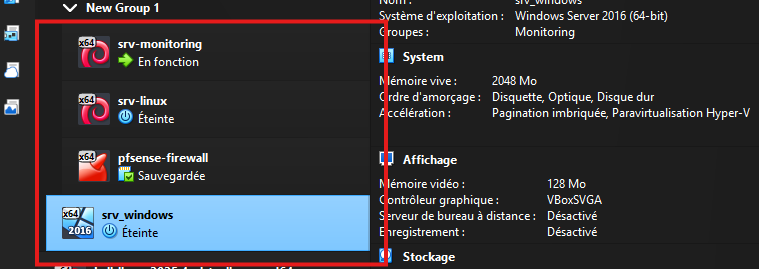
\includegraphics[width=0.85\textwidth]{images/vms_list.png}
\caption{Liste des machines virtuelles déployées dans VirtualBox}
\label{fig:vms_list}
\end{figure}

\TitreB{Plan d'adressage IP}

\begin{table}[H]
\centering
\begin{tabular}{lllll}
\toprule
\textbf{Nom d'hôte} & \textbf{Rôle} & \textbf{OS} & \textbf{IP} & \textbf{Services principaux} \\
\midrule
srv-monitoring & Supervision + SIEM & Debian 12 (GNOME) & 192.168.1.100 & Zabbix, Wazuh, MariaDB \\
srv-linux & Serveur applicatif & Debian 12 & 192.168.1.10 & Nginx, Agent Zabbix/Wazuh, SNMP \\
AK-DC & Contrôleur de domaine & Windows Server 2019 & 192.168.1.11 & AD, Agent Zabbix/Wazuh \\
firewall & Pare-feu / Routeur & pfSense 2.7.0 & 192.168.1.1 & SNMP, Syslog \\
\bottomrule
\end{tabular}
\caption{Plan d'adressage IP de l'infrastructure}
\label{tab:adressage}
\end{table}

\TitreB{Caractéristiques du réseau}

\begin{itemize}
    \item \textbf{Réseau :} 192.168.1.0/24 — Masque : 255.255.255.0
    \item \textbf{Type de réseau VirtualBox :} Bridge Adapter (accès au réseau physique)
    \item \textbf{Accès Internet :} via une deuxième interface en mode NAT (pour les téléchargements)
\end{itemize}

\TitreB{Architecture de supervision}

\begin{lstlisting}
srv-monitoring (192.168.1.100)
  |-- Supervision via Agent Zabbix --> srv-linux (192.168.1.10)
  |-- Supervision via Agent Zabbix --> AK-DC (192.168.1.11)
  |-- Supervision via SNMP v2c    --> firewall (192.168.1.1)
  |-- Collecte logs Wazuh         --> srv-linux (agent Wazuh)
  |-- Collecte logs Wazuh         --> AK-DC (agent Wazuh)
  +-- Collecte syslog             --> firewall (syslog UDP 514)
\end{lstlisting}

\newpage

%==================================================================
%  SECTION 2 — SNMP
%==================================================================
\TitreA{Configuration SNMP sur les serveurs cibles}

\TitreB{Choix de l'outil de supervision : Zabbix}

\textbf{Justification du choix :} Zabbix a été retenu pour ce TP pour les raisons suivantes :

\begin{itemize}
    \item \textbf{Open source} et sans licence commerciale, adapté à un environnement académique.
    \item \textbf{Support natif de SNMP} (v1, v2c, v3) sans plugin supplémentaire.
    \item \textbf{Templates prêts à l'emploi} pour Linux, Windows, pfSense et équipements réseau.
    \item \textbf{Agent natif} léger disponible pour Linux et Windows.
    \item \textbf{Interface web} complète pour la configuration et la visualisation.
    \item \textbf{Base de données} MariaDB/MySQL nativement supportée.
\end{itemize}

Centreon aurait été une alternative viable mais requiert plus de ressources et une courbe d'apprentissage plus importante.

\TitreB{SNMP sur srv-linux (192.168.1.10)}

\TitreC{Installation}

\begin{lstlisting}[language=bash]
sudo apt update
sudo apt install snmpd snmp -y
\end{lstlisting}

\TitreC{Configuration de /etc/snmp/snmpd.conf}

\begin{lstlisting}
# Ecouter sur toutes les interfaces
agentAddress udp:161,udp6:[::1]:161

# Communaute en lecture seule accessible depuis le reseau de supervision
rocommunity public 192.168.1.0/24

sysLocation "ESIROI"
sysContact "admin@esiroi.local"
\end{lstlisting}

\TitreC{Démarrage et vérification}

\begin{lstlisting}[language=bash]
sudo systemctl restart snmpd
sudo systemctl enable snmpd
sudo netstat -tuln | grep 161
\end{lstlisting}

\TitreC{Test de connectivité et SNMP}

\begin{figure}[H]
\centering
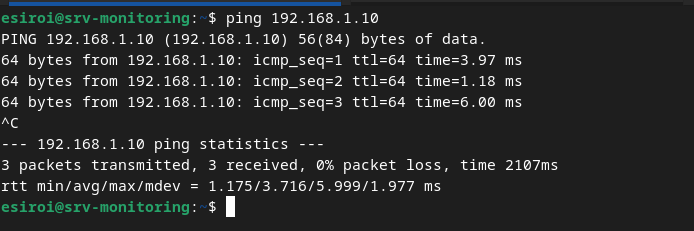
\includegraphics[width=0.85\textwidth]{images/ping_from_srv_monitoring_to_srv_linux.png}
\caption{Test de connectivité (ping) entre srv-monitoring et srv-linux}
\label{fig:ping}
\end{figure}

\TitreC{Test snmpwalk depuis srv-monitoring}

\begin{lstlisting}[language=bash]
snmpwalk -v 2c -c public 192.168.1.10
\end{lstlisting}

\textbf{Résultat obtenu :}
\begin{lstlisting}
iso.3.6.1.2.1.1.1.0 = STRING: "Linux srv-linux 6.1.0-43-amd64 ..."
iso.3.6.1.2.1.1.5.0 = STRING: "srv-linux"
...
\end{lstlisting}

\begin{figure}[H]
\centering
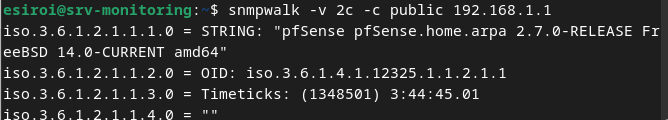
\includegraphics[width=0.85\textwidth]{images/snmp_walk_on_pfsense_result.png}
\caption{Résultat du snmpwalk sur le firewall pfSense}
\label{fig:snmpwalk}
\end{figure}

\TitreB{SNMP sur pfSense (192.168.1.1)}

La configuration SNMP sur pfSense s'effectue via l'interface web \textbf{Services → SNMP} :

\begin{itemize}
    \item Cocher \textbf{Enable the SNMP Daemon}
    \item \textbf{Polling Port :} 161 — \textbf{Community String :} \texttt{public}
    \item \textbf{Bind Interfaces :} LAN
\end{itemize}

\begin{figure}[H]
\centering
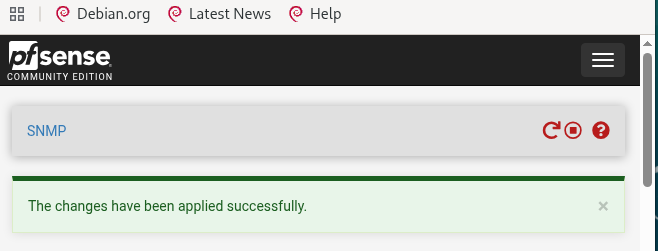
\includegraphics[width=0.85\textwidth]{images/snmp_enabled_on_pfsense.png}
\caption{Interface SNMP activée sur pfSense}
\label{fig:snmp_pfsense}
\end{figure}

\textbf{Test de validation :}
\begin{lstlisting}[language=bash]
snmpwalk -v 2c -c public 192.168.1.1
# iso.3.6.1.2.1.1.1.0 = STRING: "pfSense 2.7.0-RELEASE FreeBSD 14.0-CURRENT amd64"
\end{lstlisting}

\newpage

%==================================================================
%  SECTION 3 — SERVEUR DE SUPERVISION
%==================================================================
\TitreA{Installation et configuration du serveur de supervision}

\TitreB{Prérequis --- Système d'exploitation}

\begin{table}[H]
\centering
\begin{tabular}{ll}
\toprule
\textbf{Paramètre} & \textbf{Valeur} \\
\midrule
OS & Debian GNU/Linux 12 (Bookworm) \\
Interface graphique & GNOME (task-gnome-desktop) \\
RAM & 4 Go \\
Stockage & 50 Go \\
Réseau & Bridge Adapter (192.168.1.100) + NAT (Internet) \\
\bottomrule
\end{tabular}
\caption{Configuration de srv-monitoring}
\label{tab:srv-monitoring}
\end{table}

\textbf{Note importante :} Après l'installation de GNOME, NetworkManager a été désactivé pour éviter tout conflit avec systemd-networkd déjà en place :

\begin{lstlisting}[language=bash]
sudo systemctl stop NetworkManager
sudo systemctl disable NetworkManager
sudo systemctl restart systemd-networkd
\end{lstlisting}

\TitreB{Installation de MariaDB}

\begin{lstlisting}[language=bash]
sudo apt install -y mariadb-server
sudo systemctl start mariadb && sudo systemctl enable mariadb
sudo mysql_secure_installation
\end{lstlisting}

\TitreC{Création de la base de données Zabbix}

\begin{lstlisting}[language=sql]
CREATE DATABASE zabbix CHARACTER SET utf8mb4 COLLATE utf8mb4_bin;
CREATE USER 'zabbix'@'localhost' IDENTIFIED BY 'MotDePasseFort123!';
GRANT ALL PRIVILEGES ON zabbix.* TO 'zabbix'@'localhost';
SET GLOBAL log_bin_trust_function_creators = 1;
QUIT;
\end{lstlisting}

\begin{figure}[H]
\centering
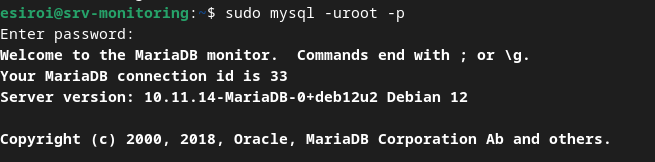
\includegraphics[width=0.85\textwidth]{images/mariadb_installed_success.png}
\caption{MariaDB installé et opérationnel}
\label{fig:mariadb}
\end{figure}

\begin{figure}[H]
\centering
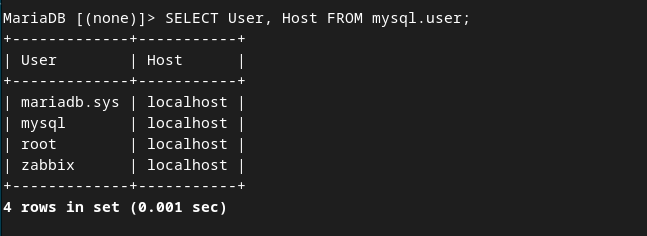
\includegraphics[width=0.85\textwidth]{images/database_schema.png}
\caption{Schéma de la base de données Zabbix importé}
\label{fig:db_schema}
\end{figure}

\begin{figure}[H]
\centering
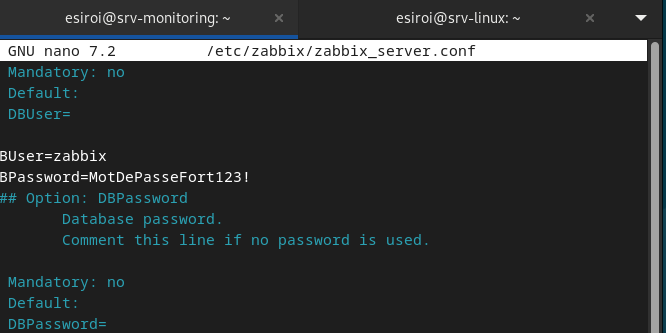
\includegraphics[width=0.85\textwidth]{images/db_password_added.png}
\caption{Mot de passe de la base de données configuré dans zabbix\_server.conf}
\label{fig:db_password}
\end{figure}

\TitreB{Installation de Zabbix Server 6.4}

\TitreC{Ajout du dépôt et installation}

\begin{lstlisting}[language=bash]
wget https://repo.zabbix.com/zabbix/6.4/debian/pool/main/z/zabbix-release/zabbix-release_6.4-1+debian12_all.deb
sudo dpkg -i zabbix-release_6.4-1+debian12_all.deb
sudo apt update
sudo apt install -y zabbix-server-mysql zabbix-frontend-php \
    zabbix-apache-conf zabbix-sql-scripts zabbix-agent
\end{lstlisting}

\TitreC{Import du schéma initial}

\begin{lstlisting}[language=bash]
sudo zcat /usr/share/zabbix-sql-scripts/mysql/server.sql.gz | mysql -uzabbix -p zabbix
sudo mysql -uroot -p -e "SET GLOBAL log_bin_trust_function_creators = 0;"
\end{lstlisting}

\TitreC{Configuration et démarrage}

\begin{lstlisting}
# /etc/zabbix/zabbix_server.conf
DBPassword=MotDePasseFort123!
\end{lstlisting}

\begin{lstlisting}[language=bash]
sudo systemctl restart zabbix-server zabbix-agent apache2
sudo systemctl enable zabbix-server zabbix-agent apache2
\end{lstlisting}

\begin{figure}[H]
\centering
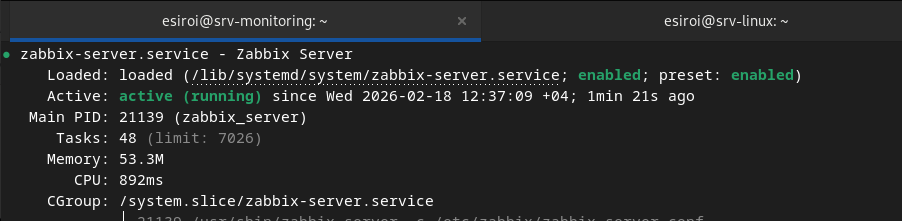
\includegraphics[width=0.85\textwidth]{images/zabbix_server_enable_activated.png}
\caption{Service Zabbix Server actif et activé au démarrage}
\label{fig:zabbix_service}
\end{figure}

\begin{figure}[H]
\centering
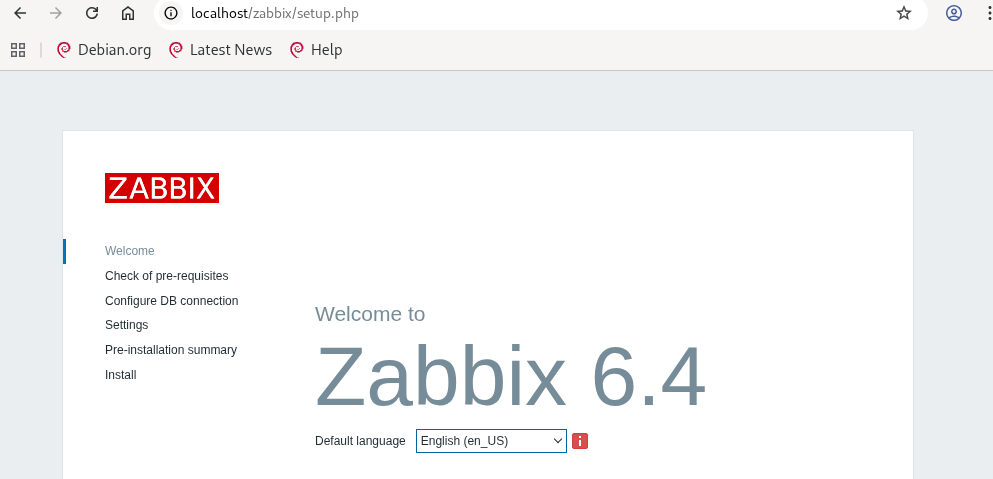
\includegraphics[width=0.85\textwidth]{images/zabbix_web_interface.png}
\caption{Interface web Zabbix accessible à \texttt{http://192.168.1.100/zabbix}}
\label{fig:zabbix_web}
\end{figure}

\newpage

%==================================================================
%  SECTION 4 — SERVEUR LINUX
%==================================================================
\TitreA{Installation et configuration du serveur Linux}

\TitreB{Prérequis}

\begin{table}[H]
\centering
\begin{tabular}{ll}
\toprule
\textbf{Paramètre} & \textbf{Valeur} \\
\midrule
OS & Debian GNU/Linux 12 (Bookworm) \\
RAM & 2 Go \\
Stockage & 20 Go \\
Adresse IP & 192.168.1.10 (statique via systemd-networkd) \\
Passerelle & 192.168.1.1 \\
\bottomrule
\end{tabular}
\caption{Configuration de srv-linux}
\label{tab:srv-linux}
\end{table}

\TitreB{Configuration de l'adresse IP statique}

\begin{lstlisting}
# /etc/systemd/network/10-static.network
[Match]
Name=enp0s8

[Network]
Address=192.168.1.10/24
Gateway=192.168.1.1
DNS=8.8.8.8
\end{lstlisting}

\TitreB{Installation de Nginx (serveur web port 80)}

\begin{lstlisting}[language=bash]
sudo apt install -y nginx
sudo systemctl start nginx && sudo systemctl enable nginx
sudo ss -tlnp | grep :80
\end{lstlisting}

\begin{figure}[H]
\centering
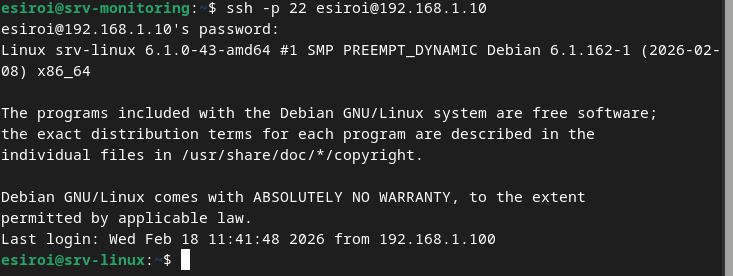
\includegraphics[width=0.85\textwidth]{images/ssh_acces_from_srv_monitoring_to_srv_linux.png}
\caption{Accès SSH depuis srv-monitoring vers srv-linux}
\label{fig:ssh}
\end{figure}

\TitreB{Installation de l'agent Zabbix}

\begin{lstlisting}[language=bash]
wget https://repo.zabbix.com/zabbix/6.4/debian/pool/main/z/zabbix-release/zabbix-release_6.4-1+debian12_all.deb
sudo dpkg -i zabbix-release_6.4-1+debian12_all.deb
sudo apt update && sudo apt install -y zabbix-agent
\end{lstlisting}

\TitreC{Configuration de /etc/zabbix/zabbix\_agentd.conf}

\begin{lstlisting}
Server=192.168.1.100
ServerActive=192.168.1.100
Hostname=srv-linux
\end{lstlisting}

\begin{lstlisting}[language=bash]
sudo systemctl restart zabbix-agent && sudo systemctl enable zabbix-agent
\end{lstlisting}

\begin{figure}[H]
\centering
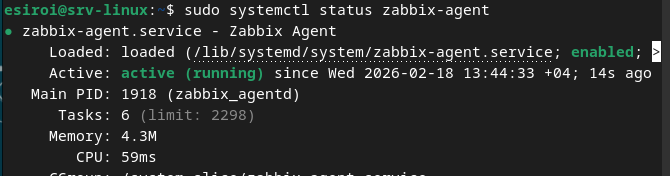
\includegraphics[width=0.85\textwidth]{images/zabbix_agent_status_on_linux_server.png}
\caption{Agent Zabbix actif sur srv-linux}
\label{fig:zabbix_agent_linux}
\end{figure}

\TitreC{Vérification depuis srv-monitoring}

\begin{lstlisting}[language=bash]
sudo apt install zabbix-get -y
zabbix_get -s 192.168.1.10 -k system.hostname
# Resultat : srv-linux
\end{lstlisting}

\begin{figure}[H]
\centering
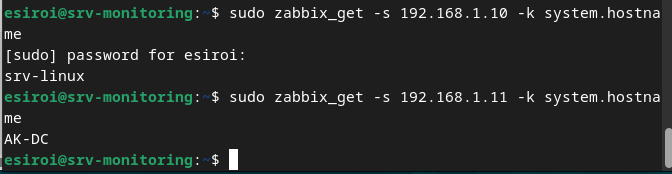
\includegraphics[width=0.85\textwidth]{images/zabbix_get_result.png}
\caption{Résultat de \texttt{zabbix\_get} confirmant la communication avec l'agent}
\label{fig:zabbix_get}
\end{figure}

\TitreB{Installation de l'agent Wazuh}

\begin{lstlisting}[language=bash]
curl -s https://packages.wazuh.com/key/GPG-KEY-WAZUH | sudo apt-key add -
echo "deb https://packages.wazuh.com/4.x/apt/ stable main" \
    | sudo tee /etc/apt/sources.list.d/wazuh.list
sudo apt update && sudo apt install -y wazuh-agent
\end{lstlisting}

\TitreC{Configuration de /var/ossec/etc/ossec.conf}

\begin{lstlisting}[language=xml]
<client>
  <server>
    <address>192.168.1.100</address>
    <port>1514</port>
    <protocol>tcp</protocol>
  </server>
</client>
\end{lstlisting}

\begin{lstlisting}[language=bash]
sudo systemctl start wazuh-agent && sudo systemctl enable wazuh-agent
\end{lstlisting}

\begin{figure}[H]
\centering
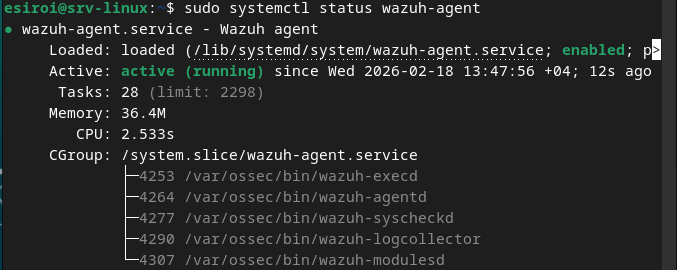
\includegraphics[width=0.85\textwidth]{images/wazuh_agent_status_on_linux_server.png}
\caption{Agent Wazuh v4.7.5 actif sur srv-linux}
\label{fig:wazuh_agent_linux}
\end{figure}

\newpage

%==================================================================
%  SECTION 5 — PFSENSE
%==================================================================
\TitreA{Configuration du pare-feu pfSense}

\TitreB{Prérequis}

\begin{table}[H]
\centering
\begin{tabular}{ll}
\toprule
\textbf{Paramètre} & \textbf{Valeur} \\
\midrule
OS & pfSense 2.7.0-RELEASE (FreeBSD 14.0-CURRENT) \\
RAM & 1 Go \\
Stockage & 12 Go \\
Interface WAN & 192.168.1.1/24 (Bridge) \\
\bottomrule
\end{tabular}
\caption{Configuration du pare-feu pfSense}
\label{tab:pfsense}
\end{table}

\TitreB{Accès à l'interface web}

\begin{lstlisting}
URL          : http://192.168.1.1
Utilisateur  : admin
Mot de passe : pfsense
\end{lstlisting}

\begin{figure}[H]
\centering
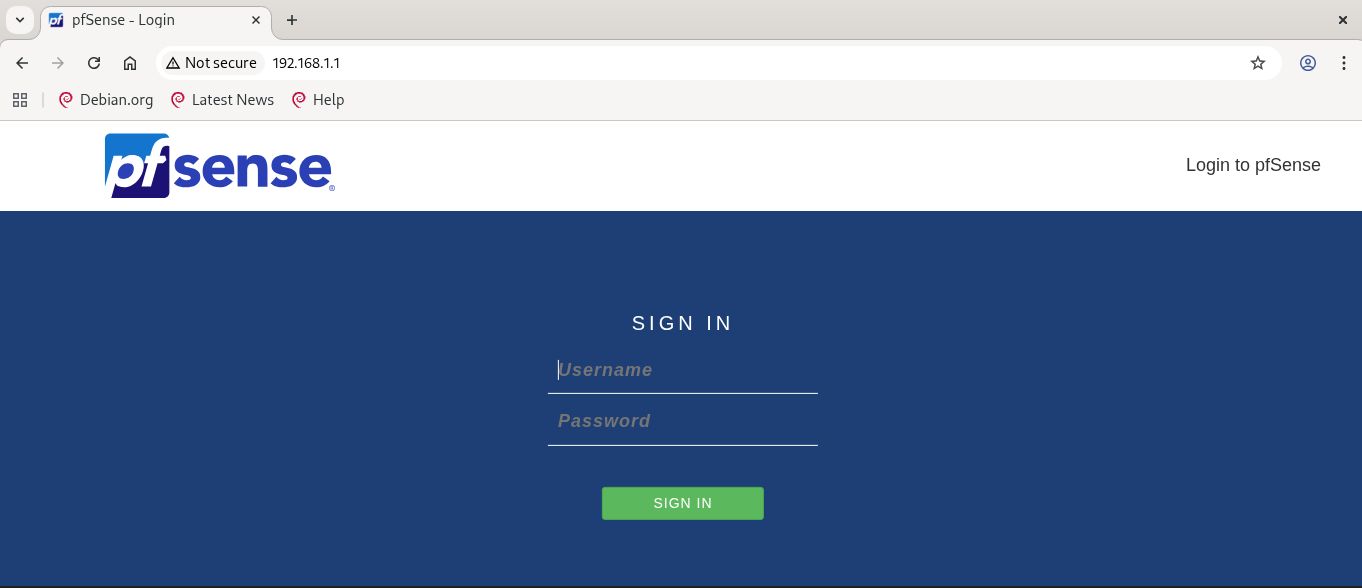
\includegraphics[width=0.85\textwidth]{images/pfsense_web_interface_login.png}
\caption{Page de connexion à l'interface web pfSense}
\label{fig:pfsense_login}
\end{figure}

\begin{figure}[H]
\centering
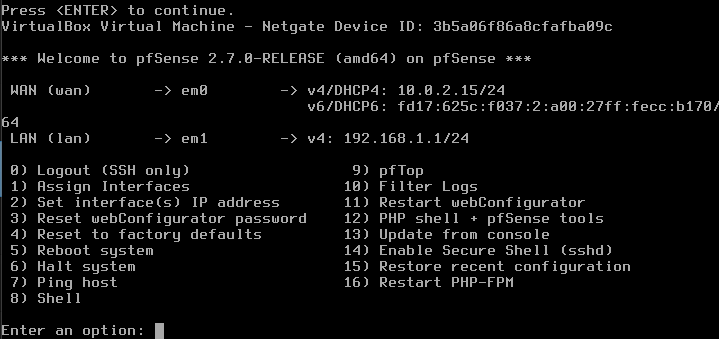
\includegraphics[width=0.85\textwidth]{images/pfsense_firewall_terminal_interface.png}
\caption{Interface console pfSense (accès terminal)}
\label{fig:pfsense_terminal}
\end{figure}

\TitreB{Configuration du transfert de logs vers Wazuh (Syslog)}

Depuis l'interface web pfSense \textbf{Status → System Logs → Settings} :

\begin{itemize}
    \item Activer \textbf{Send log messages to remote syslog server}
    \item \textbf{IP address :} 192.168.1.100 — \textbf{Port :} 514 — \textbf{Protocol :} UDP
    \item \textbf{Remote Syslog Contents :} System Events, Firewall Events
\end{itemize}

\begin{figure}[H]
\centering
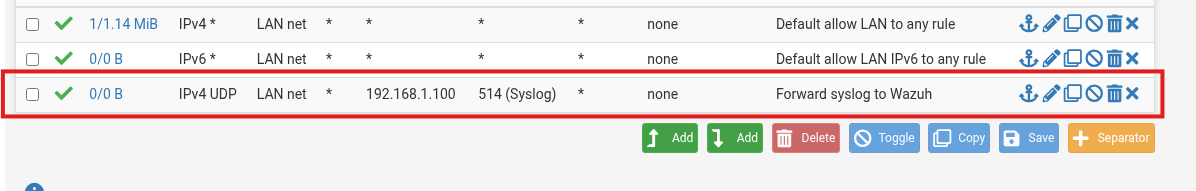
\includegraphics[width=0.85\textwidth]{images/firewall_rule_for_syslog.png}
\caption{Règle de pare-feu autorisant le transfert syslog UDP/514 vers srv-monitoring}
\label{fig:firewall_syslog}
\end{figure}

\newpage

%==================================================================
%  SECTION 6 — SERVEUR WINDOWS
%==================================================================
\TitreA{Configuration du serveur Windows}

\TitreB{Prérequis}

\begin{table}[H]
\centering
\begin{tabular}{ll}
\toprule
\textbf{Paramètre} & \textbf{Valeur} \\
\midrule
OS & Windows Server 2019 (version 10.0.17763) \\
Nom d'hôte & AK-DC \\
RAM & 4 Go — Stockage : 60 Go \\
Adresse IP & 192.168.1.11 (statique) \\
Rôle & Active Directory Domain Controller \\
\bottomrule
\end{tabular}
\caption{Configuration de AK-DC}
\label{tab:akdc}
\end{table}

\TitreB{Installation de l'agent Zabbix}

L'agent Zabbix 6.4 pour Windows a été téléchargé depuis le site officiel et installé via l'installateur MSI.

\TitreC{Configuration de zabbix\_agentd.conf}

\begin{lstlisting}
Server=192.168.1.100
ServerActive=192.168.1.100
Hostname=AK-DC
\end{lstlisting}

\TitreC{Démarrage et vérification}

\begin{lstlisting}[language=bash]
# PowerShell
Start-Service "Zabbix Agent"
Get-Service -Name "*zabbix*"
\end{lstlisting}

\begin{lstlisting}[language=bash]
# Depuis srv-monitoring
zabbix_get -s AK-DC -k system.hostname   # Resultat : AK-DC
zabbix_get -s AK-DC -k agent.version     # Resultat : 6.4.0
zabbix_get -s AK-DC -k agent.ping        # Resultat : 1
\end{lstlisting}

\TitreB{Installation de l'agent Wazuh}

L'agent Wazuh 4.7.5 pour Windows a été installé via le fichier MSI. L'emplacement de l'installation est \texttt{C:\textbackslash{}Program Files (x86)\textbackslash{}ossec-agent\textbackslash{}} (chemin hérité OSSEC).

\TitreC{Installation silencieuse}

\begin{lstlisting}
msiexec /i "%TEMP%\wazuh-agent.msi" /q
    WAZUH_MANAGER="192.168.1.100"
    WAZUH_REGISTRATION_SERVER="192.168.1.100"
    PROTOCOL=tcp
\end{lstlisting}

\TitreC{Configuration ossec.conf}

\begin{lstlisting}[language=xml]
<client>
  <server>
    <address>192.168.1.100</address>
    <manager_address>192.168.1.100</manager_address>
  </server>
</client>
\end{lstlisting}

\TitreC{Démarrage et vérification des logs}

\begin{lstlisting}
# PowerShell
Start-Service -Name "WazuhSvc"
Get-Content "C:\Program Files (x86)\ossec-agent\ossec.log" -Tail 20
# 2026/02/19 01:35:32 wazuh-agent: INFO: Started (pid: 3032).
\end{lstlisting}

\newpage

%==================================================================
%  SECTION 7 — SUPERVISION ZABBIX
%==================================================================
\TitreA{Supervision avec Zabbix}

\TitreB{Ajout des hôtes dans Zabbix}

Depuis l'interface web \texttt{http://192.168.1.100/zabbix} via \textbf{Configuration → Hôtes → Créer un hôte} :

\begin{table}[H]
\centering
\begin{tabular}{lllll}
\toprule
\textbf{Nom d'hôte} & \textbf{Interface} & \textbf{Type} & \textbf{Port} & \textbf{Template} \\
\midrule
srv-linux & 192.168.1.10 & Agent Zabbix & 10050 & Linux by Zabbix agent \\
AK-DC & 192.168.1.11 & Agent Zabbix & 10050 & Windows by Zabbix agent \\
Firewall & 192.168.1.1 & SNMPv2c & 161 & Generic SNMP / pfSense SNMP \\
\bottomrule
\end{tabular}
\caption{Hôtes configurés dans Zabbix}
\label{tab:zabbix_hosts}
\end{table}

\begin{figure}[H]
\centering
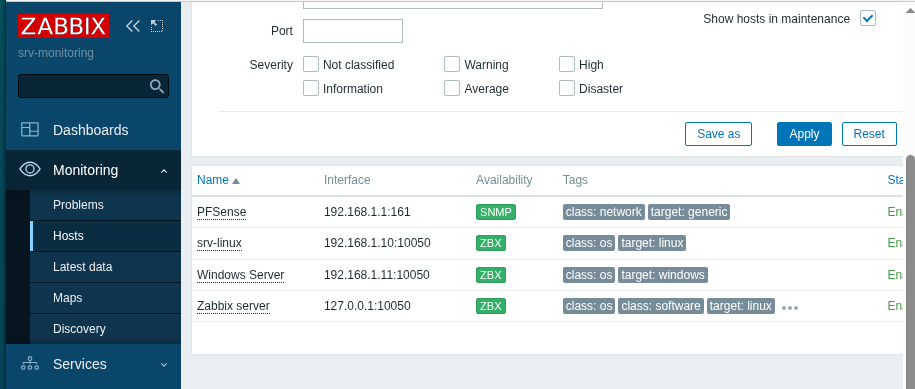
\includegraphics[width=0.85\textwidth]{images/zabbix_3_hosts_supervised.png}
\caption{Les 3 hôtes supervisés dans Zabbix : srv-linux, AK-DC et firewall}
\label{fig:zabbix_hosts}
\end{figure}

\TitreB{Vérification de la connectivité}

\begin{lstlisting}[language=bash]
# Depuis srv-monitoring
zabbix_get -s 192.168.1.10 -k system.hostname   # --> srv-linux
zabbix_get -s AK-DC -k agent.ping               # --> 1
zabbix_get -s AK-DC -k agent.version            # --> 6.4.0
snmpwalk -v 2c -c public 192.168.1.1             # --> pfSense info
snmpwalk -v 2c -c public 192.168.1.10            # --> Linux srv-linux info
\end{lstlisting}

\TitreB{Supervision SNMP avancée du firewall}

Un item SNMP a été configuré pour surveiller le trafic de l'interface WAN du firewall :

\begin{itemize}
    \item \textbf{Nom :} Interface WAN traffic
    \item \textbf{Type :} SNMP v2c
    \item \textbf{OID :} \texttt{.1.3.6.1.2.1.2.2.1.10.1} (octets entrants)
    \item \textbf{Unité :} B — \textbf{Intervalle :} 60s
\end{itemize}

\begin{figure}[H]
\centering
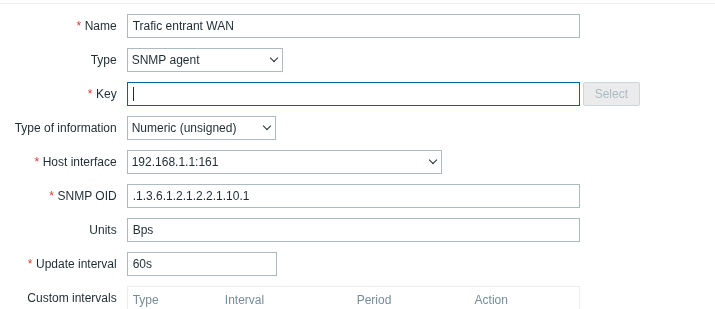
\includegraphics[width=0.85\textwidth]{images/item_config_for_snmp_wan_interface.png}
\caption{Configuration de l'item SNMP pour surveiller le trafic de l'interface WAN}
\label{fig:snmp_wan}
\end{figure}

\begin{figure}[H]
\centering
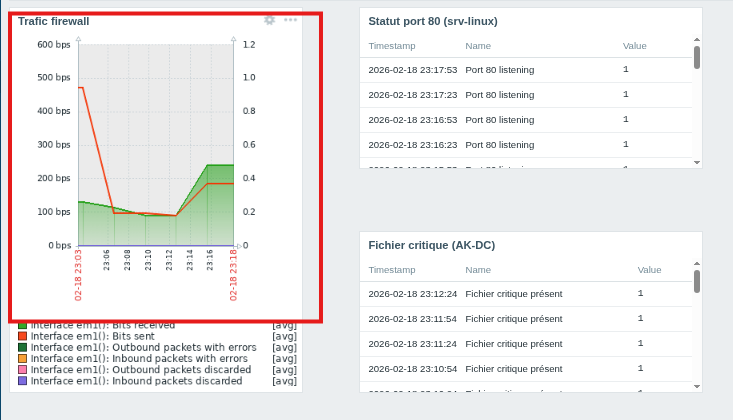
\includegraphics[width=0.85\textwidth]{images/network_trafic_after_flood_ping.png}
\caption{Trafic réseau visible dans Zabbix après un flood ping sur l'interface WAN}
\label{fig:trafic}
\end{figure}

\newpage

%==================================================================
%  SECTION 8 — SUPERVISION AVANCÉE
%==================================================================
\TitreA{Supervision avancée --- Sondes et alertes}

\TitreB{Supervision du port 80 (srv-linux)}

\TitreC{Objectif}

Détecter en temps réel si le service web Nginx est arrêté sur srv-linux et lever une alerte.

\TitreC{Création de l'item}

\begin{table}[H]
\centering
\begin{tabular}{ll}
\toprule
\textbf{Paramètre} & \textbf{Valeur} \\
\midrule
Nom & Port 80 listening \\
Type & Zabbix agent \\
Clé & \texttt{net.tcp.listen[80]} \\
Type d'information & Numeric (unsigned) \\
Intervalle & 30s \\
\bottomrule
\end{tabular}
\caption{Configuration de l'item port 80}
\label{tab:item_port80}
\end{table}

La clé \texttt{net.tcp.listen[80]} retourne \texttt{1} si le port est en écoute, \texttt{0} sinon.

\TitreC{Création du trigger}

\begin{table}[H]
\centering
\begin{tabular}{ll}
\toprule
\textbf{Paramètre} & \textbf{Valeur} \\
\midrule
Nom & Port 80 is down on srv-linux \\
Sévérité & High \\
Expression & \texttt{last(/srv-linux/net.tcp.listen[80])=0} \\
\bottomrule
\end{tabular}
\caption{Configuration du trigger port 80}
\label{tab:trigger_port80}
\end{table}

\begin{figure}[H]
\centering
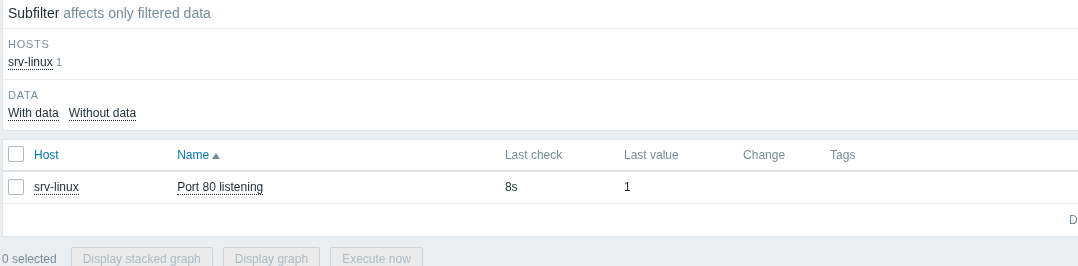
\includegraphics[width=0.85\textwidth]{images/port_80_litening_in_latest_data.png}
\caption{Valeur de l'item \texttt{net.tcp.listen[80]} dans ``Latest data'' (valeur = 1, port actif)}
\label{fig:port80_data}
\end{figure}

\begin{figure}[H]
\centering
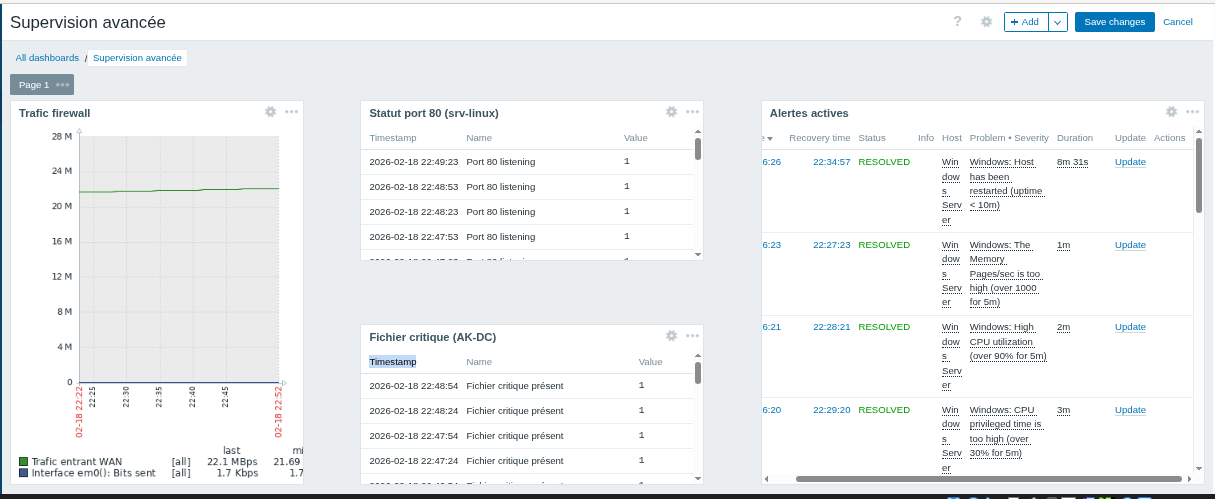
\includegraphics[width=0.85\textwidth]{images/sup_avance_dashboard_before_simulation.png}
\caption{Dashboard Zabbix avant la simulation --- aucune alerte active}
\label{fig:dashboard_before}
\end{figure}

\TitreC{Simulation de l'arrêt du service}

\begin{lstlisting}[language=bash]
# Sur srv-linux
sudo systemctl stop nginx
\end{lstlisting}

\begin{figure}[H]
\centering
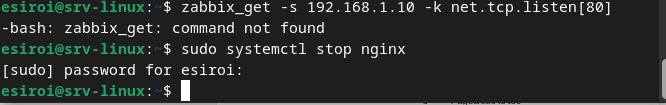
\includegraphics[width=0.85\textwidth]{images/simulation_nginx_stop.png}
\caption{Arrêt du service Nginx via \texttt{systemctl stop nginx}}
\label{fig:nginx_stop}
\end{figure}

\begin{figure}[H]
\centering
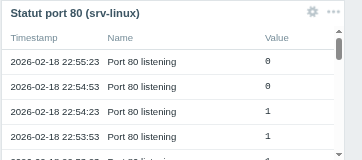
\includegraphics[width=0.85\textwidth]{images/simulation_status_port_80_0.png}
\caption{Alerte déclenchée dans Zabbix : l'item passe à 0, le trigger se déclenche}
\label{fig:port80_alert}
\end{figure}

\begin{lstlisting}[language=bash]
# Redemarrage du service
sudo systemctl start nginx
\end{lstlisting}

\TitreB{Supervision de la présence d'un fichier critique (AK-DC)}

\TitreC{Objectif}

Détecter la suppression d'un fichier critique sur le contrôleur de domaine Windows et envoyer une alerte.

\TitreC{Création du fichier surveillé}

\begin{lstlisting}
# PowerShell (admin)
New-Item -ItemType Directory -Path "C:\Supervision\" -Force
New-Item -ItemType File -Path "C:\Supervision\fichier_critique.txt" `
    -Value "Fichier de supervision ESIROI - NE PAS SUPPRIMER"
\end{lstlisting}

\TitreC{Configuration UserParameter dans zabbix\_agentd.conf}

\begin{lstlisting}
UserParameter=check.file.exists[*],powershell -Command `
    "if (Test-Path -Path '$1') { echo 1 } else { echo 0 }"
\end{lstlisting}

\begin{lstlisting}
Restart-Service "Zabbix Agent"
\end{lstlisting}

\TitreC{Item et trigger}

\begin{table}[H]
\centering
\begin{tabular}{ll}
\toprule
\textbf{Paramètre} & \textbf{Valeur} \\
\midrule
Clé item & \texttt{vfs.file.exists[C:\textbackslash{}Supervision\textbackslash{}fichier\_critique.txt]} \\
Sévérité trigger & High \\
Expression & \texttt{last(/AK-DC/vfs.file.exists[...])=0} \\
\bottomrule
\end{tabular}
\caption{Configuration de la surveillance du fichier critique}
\label{tab:fichier_critique}
\end{table}

\begin{figure}[H]
\centering
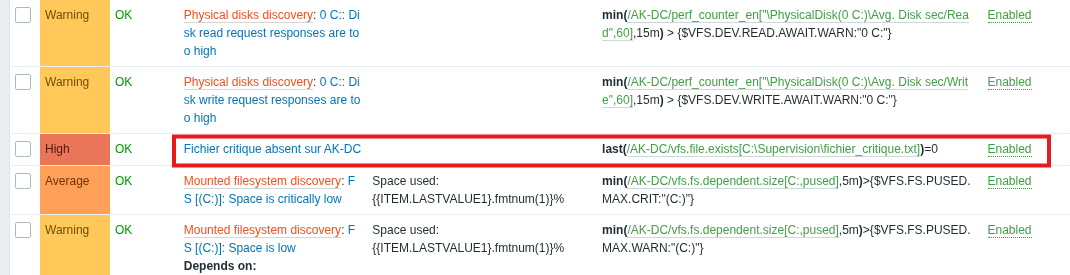
\includegraphics[width=0.85\textwidth]{images/trigger_rules_critic_files.png}
\caption{Règle de trigger configurée pour détecter l'absence du fichier critique}
\label{fig:trigger_fichier}
\end{figure}

\TitreC{Test et simulation}

\begin{lstlisting}
# PowerShell : Simuler la suppression
Remove-Item C:\Supervision\fichier_critique.txt -Force
\end{lstlisting}

\begin{figure}[H]
\centering
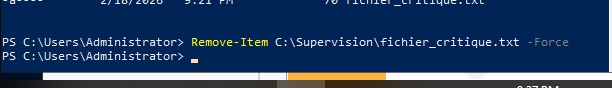
\includegraphics[width=0.85\textwidth]{images/critic_file_removed.png}
\caption{Suppression du fichier critique \texttt{C:\textbackslash{}Supervision\textbackslash{}fichier\_critique.txt}}
\label{fig:fichier_removed}
\end{figure}

\begin{figure}[H]
\centering
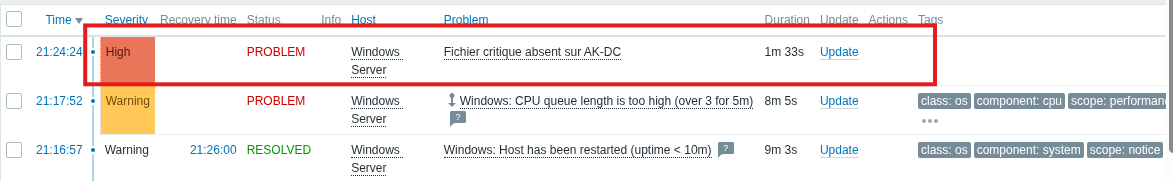
\includegraphics[width=0.85\textwidth]{images/alert_result_critic_file_removed.png}
\caption{Alerte de niveau ``High'' déclenchée dans Zabbix après la suppression}
\label{fig:alert_fichier}
\end{figure}

\begin{figure}[H]
\centering
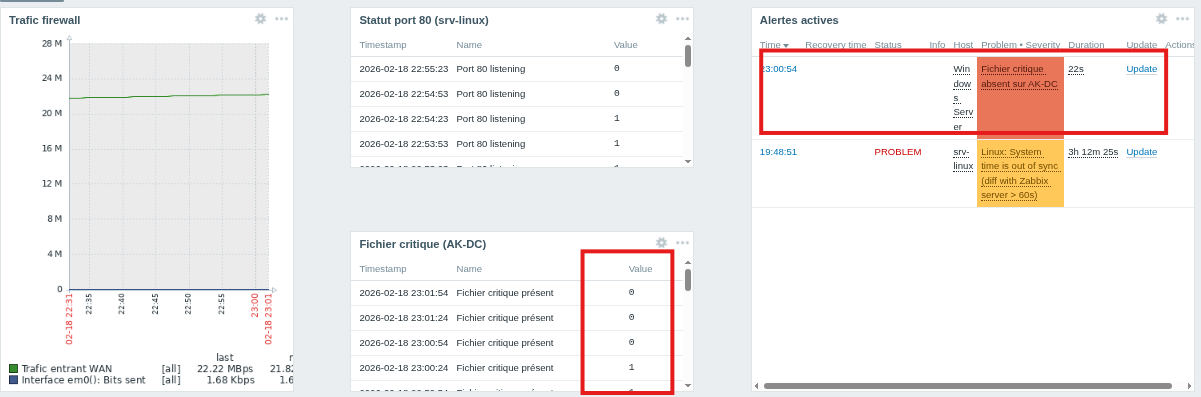
\includegraphics[width=0.85\textwidth]{images/dashboard_after_critic_file_deleted.png}
\caption{Dashboard après suppression du fichier critique : alerte active visible}
\label{fig:dashboard_alert}
\end{figure}

\begin{lstlisting}
# PowerShell : Recréer le fichier
New-Item -ItemType File -Path "C:\Supervision\fichier_critique.txt" -Value "Present"
\end{lstlisting}

\begin{figure}[H]
\centering
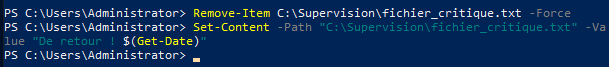
\includegraphics[width=0.85\textwidth]{images/critic_file_recreated.png}
\caption{Recréation du fichier critique sur AK-DC}
\label{fig:fichier_recreated}
\end{figure}

\begin{figure}[H]
\centering
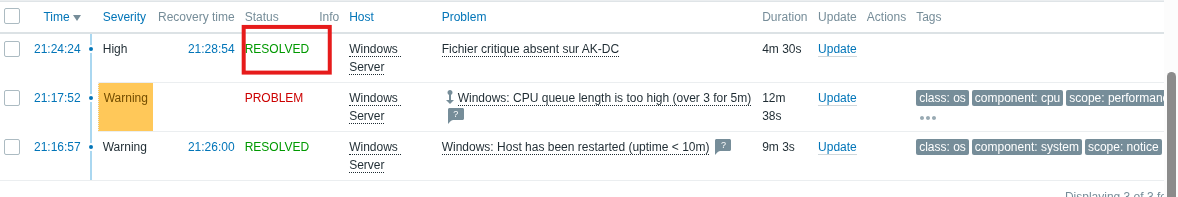
\includegraphics[width=0.85\textwidth]{images/alert_resolved_after_critic_file_back.png}
\caption{Alerte résolue automatiquement après recréation du fichier}
\label{fig:alert_resolved}
\end{figure}

\newpage

%==================================================================
%  SECTION 9 — WAZUH SIEM
%==================================================================
\TitreA{SIEM Wazuh --- Centralisation des logs}

\TitreB{Architecture Wazuh All-in-One}

Wazuh a été déployé en mode All-in-One sur \texttt{srv-monitoring} (192.168.1.100), regroupant sur une seule machine les trois composants :

\begin{itemize}
    \item \textbf{Wazuh Manager} : collecte et analyse des événements de sécurité
    \item \textbf{Wazuh Indexer} : indexation et stockage des données (basé sur OpenSearch)
    \item \textbf{Wazuh Dashboard} : interface web de visualisation
\end{itemize}

\TitreB{Installation Wazuh (All-in-One)}

\begin{lstlisting}[language=bash]
curl -sO https://packages.wazuh.com/4.7/wazuh-install.sh
chmod +x wazuh-install.sh
sudo ./wazuh-install.sh --generate-config-files
sudo ./wazuh-install.sh --wazuh-indexer node-1
sudo ./wazuh-install.sh --start-cluster
sudo ./wazuh-install.sh --wazuh-server wazuh-1
sudo ./wazuh-install.sh --wazuh-dashboard dashboard
\end{lstlisting}

\TitreC{Récupération du mot de passe admin}

\begin{lstlisting}[language=bash]
sudo tar -O -xvf wazuh-install-files.tar wazuh-install-files/wazuh-passwords.txt
\end{lstlisting}

\begin{lstlisting}
URL      : https://192.168.1.100
Login    : admin
Password : (recupere lors de l'installation)
\end{lstlisting}

\begin{figure}[H]
\centering
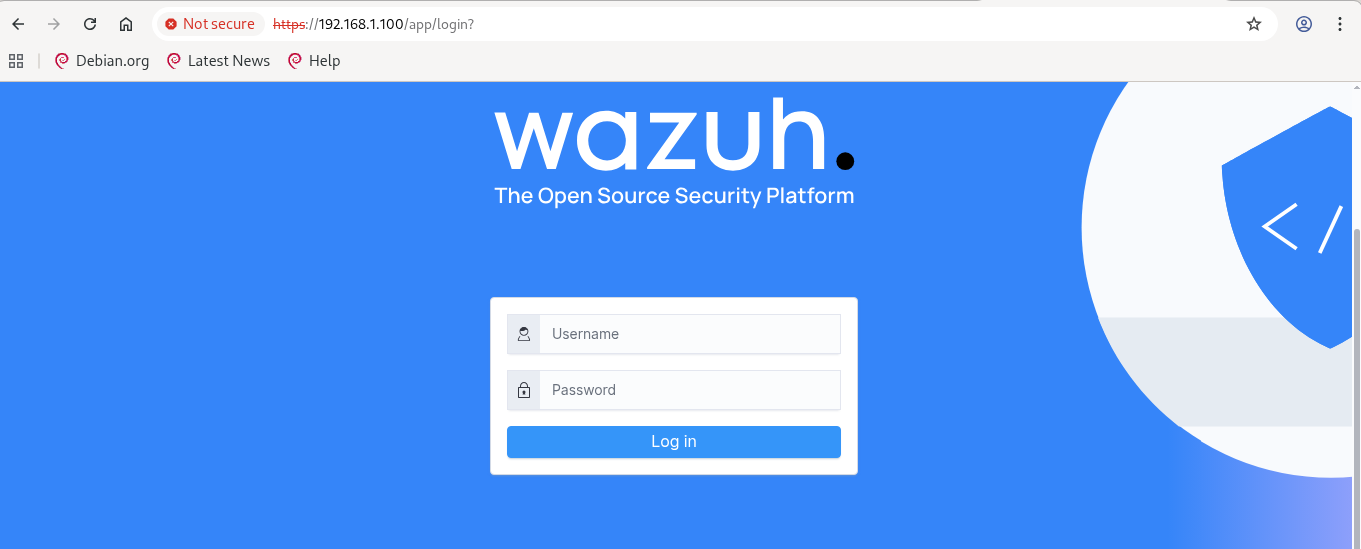
\includegraphics[width=0.85\textwidth]{images/wazuh_web_interface.png}
\caption{Interface web Wazuh Dashboard accessible à \texttt{https://192.168.1.100}}
\label{fig:wazuh_web}
\end{figure}

\begin{figure}[H]
\centering
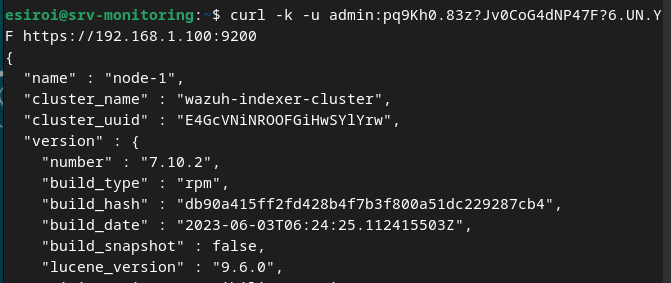
\includegraphics[width=0.85\textwidth]{images/curl_acces_on_wazuh_dashboard.png}
\caption{Vérification de l'accès HTTPS au dashboard Wazuh via curl}
\label{fig:curl_wazuh}
\end{figure}

\begin{figure}[H]
\centering
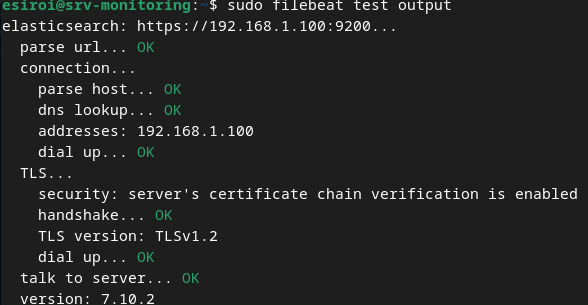
\includegraphics[width=0.85\textwidth]{images/filebeat_output_test.png}
\caption{Test de la sortie Filebeat confirmant la connexion vers le Wazuh Indexer}
\label{fig:filebeat}
\end{figure}

\TitreB{Agents Wazuh enregistrés}

Après l'installation et la configuration des agents sur srv-linux et AK-DC :

\begin{figure}[H]
\centering
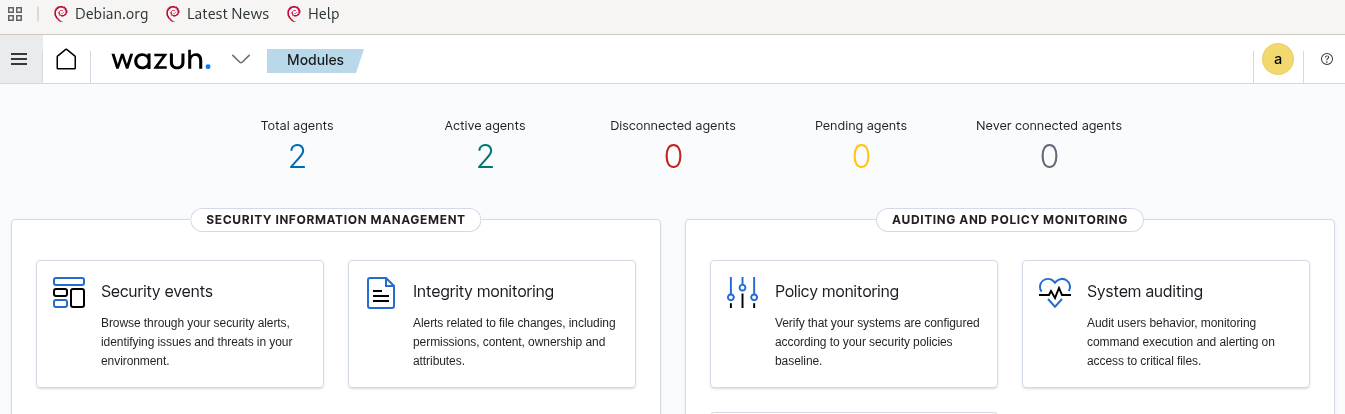
\includegraphics[width=0.85\textwidth]{images/wazuh_dashboard_agent_diplayed.png}
\caption{Agents Wazuh affichés dans le dashboard}
\label{fig:wazuh_agents}
\end{figure}

\begin{figure}[H]
\centering
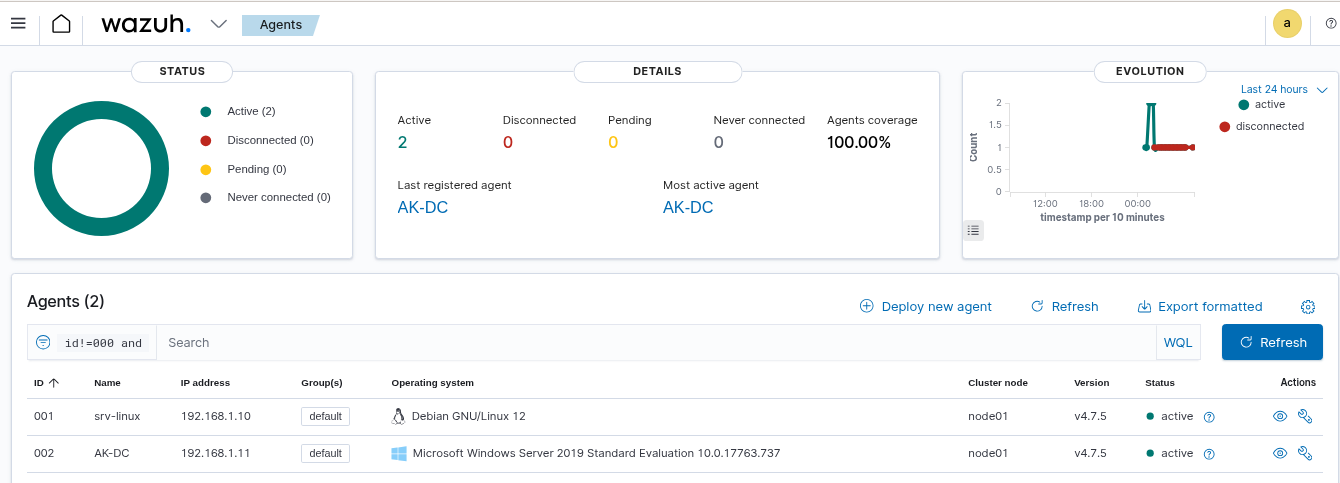
\includegraphics[width=0.85\textwidth]{images/2_agents_on_dashboard.png}
\caption{Deux agents actifs : srv-linux et AK-DC dans le tableau de bord Wazuh}
\label{fig:2agents}
\end{figure}

\begin{figure}[H]
\centering
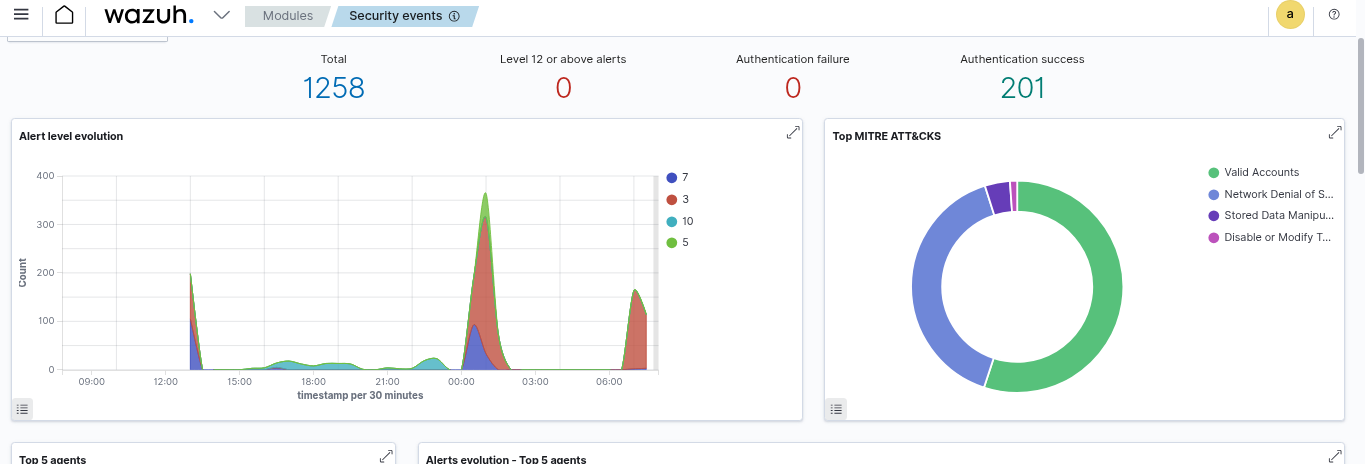
\includegraphics[width=0.85\textwidth]{images/agents_securtiy_events.png}
\caption{Événements de sécurité collectés et affichés dans le dashboard Wazuh}
\label{fig:security_events}
\end{figure}

\TitreB{Collecte des logs système}

Les agents Wazuh collectent automatiquement les journaux des systèmes supervisés.

\textbf{Sur srv-linux :} logs \texttt{/var/log/auth.log} (authentification SSH), \texttt{/var/log/syslog}, et surveillance d'intégrité de fichiers (FIM).

\textbf{Sur AK-DC (Windows) :} Event Channel System (\texttt{eventchannel}), logs d'authentification Windows et surveillance Active Directory.

\begin{lstlisting}[language=xml]
<!-- ossec.conf (AK-DC) -->
<localfile>
  <location>System</location>
  <log_format>eventchannel</log_format>
</localfile>
\end{lstlisting}

\textbf{Depuis pfSense :} logs syslog transmis en UDP/514 vers 192.168.1.100.

\newpage

%==================================================================
%  SECTION 10 — ATTAQUE BRUTE FORCE
%==================================================================
\TitreA{Simulation d'une attaque par force brute SSH}

\TitreB{Objectif}

Simuler une attaque par dictionnaire sur le service SSH de srv-linux et vérifier que Wazuh détecte et corrèle les événements dans le SIEM.

\TitreB{Préparation de l'attaque}

\TitreC{Installation de l'outil d'attaque}

\begin{lstlisting}[language=bash]
# Depuis srv-monitoring
sudo apt update && sudo apt install -y hydra
\end{lstlisting}

\TitreC{Création du dictionnaire de mots de passe}

\begin{lstlisting}[language=bash]
cat > PASSWD_LIST.txt << EOF
password
123456
admin
root
test
esiroi
debian
wrongpass
badpassword
motdepasse
passtest
lastpass
EOF
\end{lstlisting}

\TitreB{Lancement de l'attaque}

\begin{lstlisting}[language=bash]
sudo hydra -l esiroi -P PASSWD_LIST.txt 192.168.1.10 ssh
\end{lstlisting}

\textbf{Résultat de l'attaque :}
\begin{lstlisting}
[DATA] max 13 tasks per 1 server, overall 13 tasks, 13 login tries (l:1/p:13)
[DATA] attacking ssh://192.168.1.10:22/
1 of 1 target completed, 0 valid password found
\end{lstlisting}

Hydra n'a pas trouvé le mot de passe correct dans la liste (attendu), mais les tentatives d'authentification ont bien été enregistrées dans les logs de srv-linux.

\begin{figure}[H]
\centering
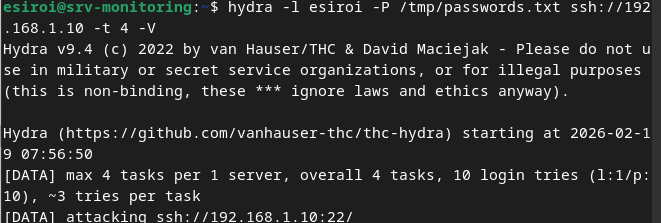
\includegraphics[width=0.85\textwidth]{images/simutation_attaque_brute_force.png}
\caption{Lancement de l'attaque par force brute SSH avec Hydra depuis srv-monitoring}
\label{fig:hydra}
\end{figure}

\TitreB{Détection par Wazuh}

Wazuh a détecté les tentatives de connexion SSH grâce aux règles de corrélation intégrées (règle 5712 --- SSH brute force).

\begin{figure}[H]
\centering
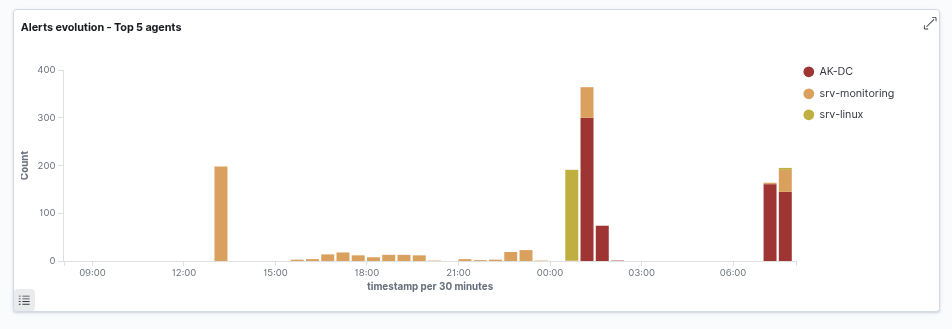
\includegraphics[width=0.85\textwidth]{images/top_5_attacks_detected_ssh_brute_force.png}
\caption{Wazuh : Top 5 des attaques détectées --- la force brute SSH apparaît en première position}
\label{fig:wazuh_bruteforce}
\end{figure}

\TitreB{Analyse dans le Dashboard Wazuh}

Dans le Dashboard Wazuh → \textbf{Threat Hunting} → \textbf{srv-linux} :

\begin{itemize}
    \item Augmentation significative des événements ``Authentication Failure''
    \item Corrélation des tentatives multiples depuis la même source (192.168.1.100)
    \item Classification automatique de l'attaque comme \textbf{brute force SSH}
    \item Règle MITRE ATT\&CK associée : \textbf{T1110 --- Brute Force} \cite{mitre_t1110}
\end{itemize}

Ce résultat confirme l'efficacité du SIEM pour détecter des attaques en temps réel, même sans intervention manuelle.

\newpage

%==================================================================
%  SECTION 11 — CONCLUSION
%==================================================================
\TitreA{Conclusion}

\TitreB{Bilan des réalisations}

Ce travail pratique a permis de déployer et de valider une infrastructure complète de supervision et de sécurité réseau, intégrant les outils professionnels Zabbix \cite{zabbix64} et Wazuh \cite{wazuh_install}.

\begin{itemize}
    \item \textbf{Étape 1 --- Infrastructure de base :} déploiement des 4 VMs, configuration réseau \texttt{192.168.1.0/24} en mode Bridge, SNMP configuré sur srv-linux et pfSense \cite{snmp_rfc}, Zabbix 6.4 installé avec MariaDB \cite{mariadb_docs}, 3 hôtes supervisés dans le tableau de bord.

    \item \textbf{Étape 2 --- Supervision avancée :} item \texttt{net.tcp.listen[80]} sur srv-linux avec trigger et alerte testés, item \texttt{vfs.file.exists} sur AK-DC avec simulation de suppression et validation de l'alerte \cite{zabbix_agent_linux}.

    \item \textbf{Étape 3 --- Centralisation des logs :} Wazuh All-in-One installé, agents v4.7.5 déployés sur srv-linux et AK-DC \cite{wazuh_agent_windows}, logs pfSense via syslog UDP/514, événements indexés dans le Dashboard Wazuh.

    \item \textbf{Étape 4 --- Simulation d'attaque :} attaque SSH par force brute (Hydra) \cite{hydra_tool} détectée et corrélée automatiquement par Wazuh, classification MITRE ATT\&CK T1110 validée \cite{wazuh_bruteforce}.
\end{itemize}

\TitreB{Points techniques notables}

\begin{itemize}
    \item La gestion du réseau via \texttt{systemd-networkd} a nécessité de désactiver NetworkManager après l'installation de GNOME pour éviter les conflits.
    \item L'agent Wazuh sur Windows Server était installé dans le chemin non standard \texttt{C:\textbackslash{}Program Files (x86)\textbackslash{}ossec-agent\textbackslash{}} (héritage OSSEC), ce qui a nécessité un diagnostic approfondi.
    \item Le renommage de l'hôte Windows de \texttt{srv-windows} en \texttt{AK-DC} dans Zabbix a résolu les erreurs de correspondance de hostname entre l'agent et le serveur.
\end{itemize}

\TitreB{Perspectives}

Cette infrastructure constitue une base solide pour aller plus loin : mise en place de SNMPv3 (chiffrement et authentification) \cite{snmp_rfc}, configuration d'alertes par email, intégration de tableaux de bord personnalisés Grafana, et déploiement d'un système de réponse automatique aux incidents (Active Response Wazuh) \cite{wazuh_bruteforce}.

\newpage

%==================================================================
%  BIBLIOGRAPHIE
%==================================================================
\section*{Bibliographie}
\addcontentsline{toc}{section}{Bibliographie}
\nocite{*}
\printbibliography[heading=none]

%==================================================================
%  PAGE DE CLÔTURE
%==================================================================
\ClotureRapport

\end{document}